%% LyX 2.2.1 created this file.  For more info, see http://www.lyx.org/.
%% Do not edit unless you really know what you are doing.
\documentclass[oneside,french,a4paper,twoside,11pt,latin9]{book2}
\usepackage[T1]{fontenc}
\usepackage[utf8]{inputenc}
\setcounter{secnumdepth}{3}
\setcounter{tocdepth}{3}
\usepackage{graphicx}

\makeatletter
%%%%%%%%%%%%%%%%%%%%%%%%%%%%%% User specified LaTeX commands.
\usepackage{these}
\usepackage{eso-pic} % image de fond, a declarer avant graphicx
%\usepackage{graphicx}
\usepackage{amssymb,amsmath,amsthm}
\usepackage{amsfonts}
\usepackage{color}
\usepackage{rotating}
\usepackage{multirow}
\usepackage{tabularx}
\usepackage[absolute]{textpos}
\usepackage{floatflt}
\usepackage{supertabular}
\usepackage{fancyhdr}
\usepackage{cite}
\usepackage{url}
\usepackage{psfrag}
\usepackage{algorithmic}
\usepackage{algorithm}
\usepackage{setspace}
\usepackage{mathrsfs}
\usepackage{lscape}
\usepackage{textcomp}
\usepackage{enumerate} 	% Modification du style possible
\usepackage{mathbbol} 	% pour les lettres avec des barres
%\usepackage{subfig}
\usepackage{subfigure} 	

\makeatother

\usepackage{babel}
\makeatletter
\addto\extrasfrench{%
   \providecommand{\og}{\leavevmode\flqq~}%
   \providecommand{\fg}{\ifdim\lastskip>\z@\unskip\fi~\frqq}%
}

\makeatother
\begin{document}
%%%%%%%%%%%%%%%%%%%%%%%%%%%%%%%%%%%%%%%%%%%%%%%%%%%%%


\pagestyle{fancy} \fancyhf{}
\fancyhead[RE]{\nouppercase{\textit{\leftmark}}} 	% Right even
\fancyhead[LO]{\nouppercase{\textit{\rightmark}}} % Left odd
\fancyhead[LE]{\textbf{\thepage}}% 								% Left even
\fancyhead[RO]{\textbf{\thepage}}% 								% Right odd
\renewcommand{\footrulewidth}{0pt}
\setlength{\headheight}{27.2pt}


%%%%%%%%%%%%%%%%%%%% Page de couverture %%%%%%%%%%%%%%%%%%%%%%%%%%
\begin{titlepage}
%%----------------------------------------------------------------------------
%% Page de Couverture 
%%----------------------------------------------------------------------------

\def\auteur{MOI}
\def\upmc{Université Pierre et Marie Curie}
\def\UPMC{\MakeUppercase{\upmc}}
\def\specialite{Spécialité : Robotique}
\def\uvsq{Université de Versailles Saint-Quentin}
%\def\sujet{Haptique Moléculaire}
\def\date{??? ??? 201?}
\def\soutenue{Soutenue le \date}
\def\asoutenir{soutenance prévue le \date}

%%----------------------------------------------------------------------------

\newcommand{\Exa}{Examinateur}
\newcommand{\Exae}{Examinatrice}
\newcommand{\Rap}{Rapporteur}
\newcommand{\Rape}{Rapporteuse}
\newcommand{\hs}{\hspace{-1cm}}

%\thispagestyle{empty}
\vspace*{-80pt}
\vspace{10mm}

\begin{center}
{\Huge \bf Thèse}\\
\end{center}

%\vspace{6pt}
%\vspace{3pt}

\begin{center}
{présentée à} \\
\end{center}

%\vspace{6pt}
%\vspace{3pt}

\begin{center}
{\large \bf L'\upmc}\\
\end{center}

%\vspace{6pt}
%\vspace{3pt}

\begin{center}
{par}\\
\end{center}

%\vspace{6pt}
%\vspace{3pt}

\begin{center}
{\large \bf \auteur}\\
\end{center}

%\vspace{6pt}
%\vspace{3pt}

\begin{center}
pour obtenir le diplôme de\\
\vspace{6pt}
{\Large \bf Doctorat de l'Universit\'e \vspace{2pt} Pierre et Marie Curie}\\
%{\Large \bf DOCTORAT DE L'UNIVERSIT\'E \vspace{2pt}\\ PIERRE ET MARIE CURIE}\\
\end{center}

%\vspace{6pt}
%\vspace{3pt}

\begin{center}
{\normalsize {\bf \specialite}}\\
\end{center}

\vspace{62pt}
%\vspace{3pt}

%\begin{center}
%\rule[1mm]{60mm}{0.2mm}\\
%\vspace{6pt}
%
%{\Large \bf \sujet}
%
%\rule[1mm]{60mm}{0.2mm}\\
%\end{center}


\begin{center}
\rule[2mm]{60mm}{0.2mm}\\
%{\Large \bf Manipulation et caract\'erisation de films fins\\}
{\Large \bf Titre qui va bien\\}
 \rule[-2mm]{60mm}{0.2mm}\\
\end{center}


\vspace{2pt}


\begin{center}
{\it \large \asoutenir}\\
\end{center}

\vspace{2pt}

\begin{center}
{\bf JURY}\\
\vspace{10pt}
{\small 
\begin{tabular}{p{0.8cm}p{3cm}p{11cm}p{1.95cm}}
%\centering
%\begin{tabular}{llll}
 \hs M.	& \hs ???   & \hs Professeur à ??? 				& \hs \Rap  \\
 \hs M. & \hs ??? 	& \hs Professeur à ???				& \hs \Rap  \\

% \hs M.	& \hs ???   & \hs Maître de conférences à l'\uvsq 	& \hs \Exa  \\  
% \hs M. & \hs ???   & \hs Maître de conférences à l'\upmc           & \hs \Exa\\
 \hs  M. 	& \hs S. REGNIER  	& \hs Directeur de thèse             																&  \\
     			&               			& \hs Professeur à l'\upmc 												& \hs \Exa  \\
\hs M.	& \hs ???     	& \hs Professeur à l'\upmc 				& \hs \Exa  \\

     			%%%%%%%%%%%%%%%%%%%%%%%%%%%%
\end{tabular}
}
\end{center}


\end{titlepage}
\cleardoublepage
%\begin{titlepage}
%%%----------------------------------------------------------------------------
%% Page de Couverture 
%%----------------------------------------------------------------------------

\def\auteur{MOI}
\def\upmc{Université Pierre et Marie Curie}
\def\UPMC{\MakeUppercase{\upmc}}
\def\specialite{Spécialité : Robotique}
\def\uvsq{Université de Versailles Saint-Quentin}
%\def\sujet{Haptique Moléculaire}
\def\date{??? ??? 201?}
\def\soutenue{Soutenue le \date}
\def\asoutenir{soutenance prévue le \date}

%%----------------------------------------------------------------------------

\newcommand{\Exa}{Examinateur}
\newcommand{\Exae}{Examinatrice}
\newcommand{\Rap}{Rapporteur}
\newcommand{\Rape}{Rapporteuse}
\newcommand{\hs}{\hspace{-1cm}}

%\thispagestyle{empty}
\vspace*{-80pt}
\vspace{10mm}

\begin{center}
{\Huge \bf Thèse}\\
\end{center}

%\vspace{6pt}
%\vspace{3pt}

\begin{center}
{présentée à} \\
\end{center}

%\vspace{6pt}
%\vspace{3pt}

\begin{center}
{\large \bf L'\upmc}\\
\end{center}

%\vspace{6pt}
%\vspace{3pt}

\begin{center}
{par}\\
\end{center}

%\vspace{6pt}
%\vspace{3pt}

\begin{center}
{\large \bf \auteur}\\
\end{center}

%\vspace{6pt}
%\vspace{3pt}

\begin{center}
pour obtenir le diplôme de\\
\vspace{6pt}
{\Large \bf Doctorat de l'Universit\'e \vspace{2pt} Pierre et Marie Curie}\\
%{\Large \bf DOCTORAT DE L'UNIVERSIT\'E \vspace{2pt}\\ PIERRE ET MARIE CURIE}\\
\end{center}

%\vspace{6pt}
%\vspace{3pt}

\begin{center}
{\normalsize {\bf \specialite}}\\
\end{center}

\vspace{62pt}
%\vspace{3pt}

%\begin{center}
%\rule[1mm]{60mm}{0.2mm}\\
%\vspace{6pt}
%
%{\Large \bf \sujet}
%
%\rule[1mm]{60mm}{0.2mm}\\
%\end{center}


\begin{center}
\rule[2mm]{60mm}{0.2mm}\\
%{\Large \bf Manipulation et caract\'erisation de films fins\\}
{\Large \bf Titre qui va bien\\}
 \rule[-2mm]{60mm}{0.2mm}\\
\end{center}


\vspace{2pt}


\begin{center}
{\it \large \asoutenir}\\
\end{center}

\vspace{2pt}

\begin{center}
{\bf JURY}\\
\vspace{10pt}
{\small 
\begin{tabular}{p{0.8cm}p{3cm}p{11cm}p{1.95cm}}
%\centering
%\begin{tabular}{llll}
 \hs M.	& \hs ???   & \hs Professeur à ??? 				& \hs \Rap  \\
 \hs M. & \hs ??? 	& \hs Professeur à ???				& \hs \Rap  \\

% \hs M.	& \hs ???   & \hs Maître de conférences à l'\uvsq 	& \hs \Exa  \\  
% \hs M. & \hs ???   & \hs Maître de conférences à l'\upmc           & \hs \Exa\\
 \hs  M. 	& \hs S. REGNIER  	& \hs Directeur de thèse             																&  \\
     			&               			& \hs Professeur à l'\upmc 												& \hs \Exa  \\
\hs M.	& \hs ???     	& \hs Professeur à l'\upmc 				& \hs \Exa  \\

     			%%%%%%%%%%%%%%%%%%%%%%%%%%%%
\end{tabular}
}
\end{center}


%\end{titlepage}
%\cleardoublepage

%%%%%%%%%%%%%%%%%%%% Fin page de couverture %%%%%%%%%%%%

%%%%%%%%%%%%%%%%%%% Resume %%%%%%%%%%%%%%%%%%%%%%%%%%%%%%%%%%%%%%%%
\thispagestyle{empty}


\noindent \normalsize \textbf{Titre qui va bien}

\noindent \scshape{\textbf{ \slshape Résumé}}

\normalfont \small 
Bla bla bla bla blabla bla bla.

\textbf{Mots clefs : }  sonde locale, haute fréquence, réalité virtuelle, caractérisation,  plateforme, milieu liquide
% 6



\vspace{24pt}

%\noindent \normalsize \textbf{Title what right fits}

\noindent \scshape{\textbf{ \slshape Abstract}}

\normalfont \small 
Blabber blabber blabber bladdeber blabber.

\textbf{Keywords: } AFM, high frequency, virtual reality, characterization, platform, liquid environment

\normalfont \normalsize
\cleardoublepage
%%%%%%%%%%%%%%%%%%% Fin de resume %%%%%%%%%%%%%%%%%%%%%%%%%%%%%%%%%



%%%%%%%%%%%%%%%%%%%% Remerciements %%%%%%%%%%%%%%%%%%%%%%%%%%%%%%%%%
\chapter*{Remerciements}
\fancyhead[LE]{} 	% Right even
 \fancyhead[RE]{\nouppercase{\textit{Remerciements}}} 	% Right even
 \thispagestyle{empty}
% 	\input{remerciements/remerciements.tex}
 \cleardoublepage 
 \fancyhead[RE]{\nouppercase{\textit{\leftmark}}} 	% Right even
 \fancyhead[LE]{\textbf{\thepage}}% 								% Left even
%%%%%%%%%%%%%%%%%%%% Fin de remerciements %%%%%%%%%%%%%%%%%%%%%%%%%%
%
\setcounter{page}{1}
\pagenumbering{roman} %pour la numerotation des page en chiffres romains
%
{
%%%%%%%%%%%%%%%%%%%% Table des matieres et des figures %%%%%%%%%%%%%%
\setlength{\parskip}{0pt}
\addcontentsline{toc}{chapter}{Table des matières}
\tableofcontents
\cleardoublepage
\addcontentsline{toc}{chapter}{Table des figures}
\listoffigures
\cleardoublepage
%%%%%%%%%%%%%%%%%%%% Fin table des matieres et des figures %%%%%%%%%%%
}



\setcounter{page}{1}
\pagenumbering{arabic}  %pour la numerotation des page en chiffres arabes




\chapter{Intro}

Lorem ipsum dolor sit amet, consectetur adipiscing elit. Proin fringilla
nisi nec lectus faucibus, id eleifend eros dignissim. Curabitur ultricies
dui ut ipsum porttitor, et fermentum diam lobortis. Pellentesque ornare
felis et enim molestie varius. Ut neque lectus, lobortis eu venenatis
et, iaculis at nulla. Suspendisse dolor sem, vulputate eu volutpat
vitae, semper in neque. Cras cursus egestas lacinia. Nunc eu tincidunt
turpis, ut placerat nibh. Nullam a urna eros. Nunc odio ipsum, luctus
et ligula vitae, iaculis iaculis ligula. Fusce suscipit ultricies
magna, id pretium enim rutrum eu. Vestibulum vehicula eu nulla in
elementum. Nunc at convallis velit. Mauris non arcu neque. Integer
eu mauris justo. Sed sed enim et magna posuere eleifend. Nam elementum
varius est non maximus.

\begin{figure}
\begin{centering}
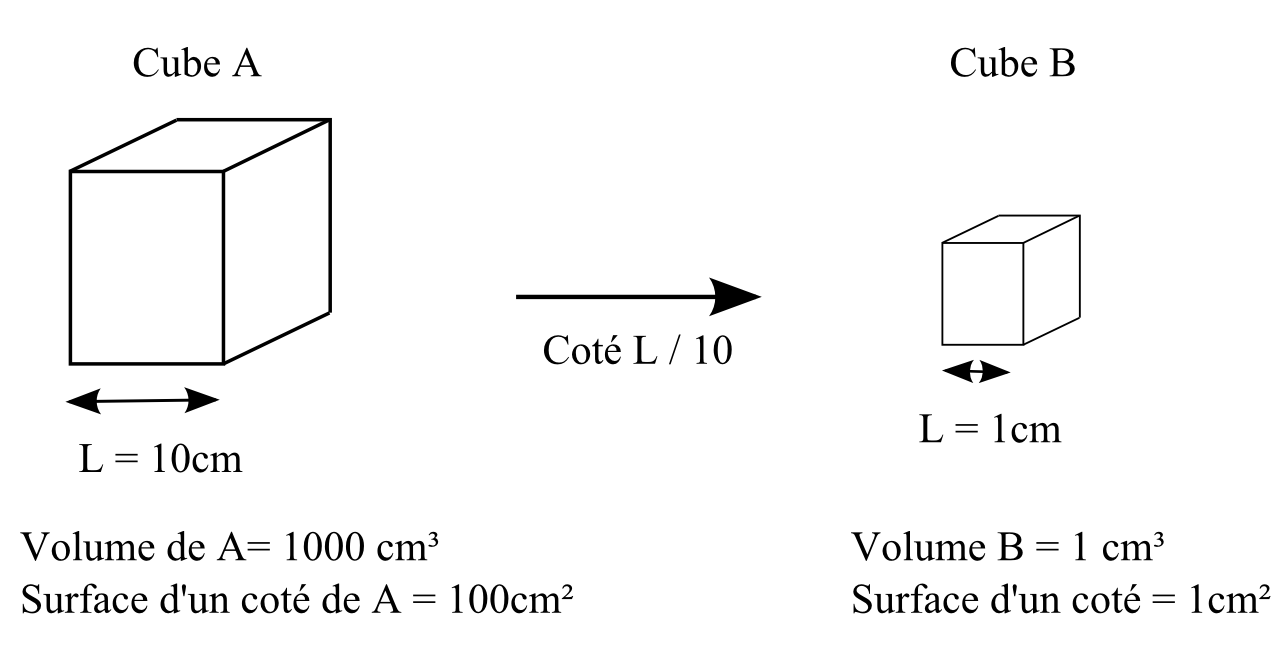
\includegraphics[width=0.75\textwidth]{chapitre1/photo_chap1/cube}
\par\end{centering}
\caption{Image}

\end{figure}

Pellentesque a euismod nibh. Vivamus erat urna, efficitur sit amet
sapien consequat, interdum dignissim dolor. Pellentesque ornare lorem
sit amet diam mollis, id eleifend arcu consectetur. Pellentesque neque
elit, mattis in leo ut, sagittis ultricies neque. Fusce vel turpis
lectus. Curabitur dolor magna, viverra a sapien sit amet, gravida
efficitur ante. Suspendisse id libero id ante vehicula vulputate.
Integer consequat sed lectus nec tristique. Aliquam erat volutpat.
Integer efficitur, elit vel tincidunt molestie, nulla purus consequat
lorem, vitae aliquam dolor lorem non nibh. Etiam lobortis leo sed
ipsum eleifend fermentum. Vivamus auctor ultricies nisi, in efficitur
lectus semper tincidunt. Maecenas sodales felis eget augue fringilla,
quis aliquet purus ultrices.

Curabitur cursus viverra enim, et fermentum tortor bibendum non. Vestibulum
non pharetra diam, sed ultrices tortor. Fusce eleifend efficitur eros,
in semper justo porttitor vitae. Ut et ligula convallis, tristique
sem ac, facilisis libero. Vestibulum quis posuere quam, lacinia varius
dui. Cum sociis natoque penatibus et magnis dis parturient montes,
nascetur ridiculus mus. Praesent maximus iaculis ipsum, ac cursus
orci. Quisque mattis mi neque, imperdiet auctor arcu posuere sagittis.
Mauris ut consectetur arcu. Aliquam ornare quis erat sit amet pretium.
Cras euismod dignissim diam ut tempus. Nunc lacus justo, posuere eu
mauris sed, mattis ultricies libero. Sed magna justo, varius a dapibus
vel, pellentesque aliquet ipsum. In iaculis volutpat nisl nec cursus.

Etiam tempor porttitor vestibulum. Pellentesque rhoncus tincidunt
libero eu scelerisque. Vivamus quis orci sit amet nisl elementum iaculis
id et justo. Duis vel mi et erat pellentesque semper ut in elit. Sed
nec congue magna. Suspendisse quis rhoncus libero. Fusce lacinia erat
vel mi sagittis laoreet. Donec ullamcorper quam sed libero gravida
ultrices. Sed auctor nibh justo, auctor vehicula mauris viverra laoreet.
In fermentum libero ac nulla mattis, vel commodo ligula dignissim.

Donec vitae porttitor neque. Aliquam finibus lobortis hendrerit. Cras
fringilla enim mauris, in bibendum risus cursus non. Aliquam at lobortis
nisl. Aliquam id sem ac mi tempus porttitor quis id tortor. Proin
rutrum varius vehicula. Cras viverra metus sed ultrices ultricies.
Sed facilisis sodales malesuada. Cras commodo nunc at finibus mollis.
Donec a est ligula.

Duis libero felis, facilisis non turpis non, mollis facilisis ante.
Morbi fringilla, est congue dignissim hendrerit, quam elit lacinia
sapien, quis cursus tortor ante eu erat. Nam semper tellus id orci
pharetra, a dapibus tortor aliquet. In dictum lacus est. Vestibulum
eleifend fringilla lorem, mollis scelerisque risus hendrerit sit amet.
Vivamus venenatis eu leo sit amet ornare. Curabitur hendrerit pharetra
purus, sed lacinia felis molestie ac.

Donec auctor est bibendum magna tempus, ac porta mi pharetra. In vel
efficitur lorem. Morbi accumsan erat ut tortor condimentum, at ornare
nibh euismod. Nam et lacus vel tellus rutrum auctor ut vel eros. Nunc
dapibus auctor hendrerit. Mauris viverra lorem dolor, nec mollis libero
interdum in. Mauris at tortor nunc. Vivamus et sem nunc. Aenean hendrerit
euismod vestibulum. Donec tincidunt eget nulla eu mattis. Ut nunc
urna, facilisis at libero sit amet, vehicula condimentum risus. Etiam
velit mauris, porttitor in dapibus sit amet, dapibus nec libero. Sed
vel sem dignissim, euismod mauris nec, dapibus nisl. Integer nec finibus
lectus.

Aliquam sit amet lorem ac elit blandit porta eget ac eros. Morbi interdum
hendrerit augue, id vehicula tortor suscipit in. Curabitur neque nisi,
sodales ut eros vel, sodales blandit nisi. Etiam vulputate quis justo
at elementum. Proin volutpat mauris facilisis lectus fermentum laoreet.
Nunc euismod velit in lorem mollis, quis feugiat velit fringilla.
Nam pretium eu magna non ornare. Integer vel libero diam. Maecenas
cursus consequat luctus. In mollis imperdiet lectus id tempor. Vestibulum
ante ipsum primis in faucibus orci luctus et ultrices posuere cubilia
Curae; Cras dignissim elit ipsum, ut finibus est feugiat ut. Praesent
vel est vitae justo aliquet hendrerit vitae eu nunc. Vestibulum quis
est magna. Vestibulum ante ipsum primis in faucibus orci luctus et
ultrices posuere cubilia Curae;



\chapter{Etat de l'art}

\cite{weill-duflos_optimizing_2015}

Lorem ipsum dolor sit amet, consectetur adipiscing elit. Proin fringilla
nisi nec lectus faucibus, id eleifend eros dignissim. Curabitur ultricies
dui ut ipsum porttitor, et fermentum diam lobortis. Pellentesque ornare
felis et enim molestie varius. Ut neque lectus, lobortis eu venenatis
et, iaculis at nulla. Suspendisse dolor sem, vulputate eu volutpat
vitae, semper in neque. Cras cursus egestas lacinia. Nunc eu tincidunt
turpis, ut placerat nibh. Nullam a urna eros. Nunc odio ipsum, luctus
et ligula vitae, iaculis iaculis ligula. Fusce suscipit ultricies
magna, id pretium enim rutrum eu. Vestibulum vehicula eu nulla in
elementum. Nunc at convallis velit. Mauris non arcu neque. Integer
eu mauris justo. Sed sed enim et magna posuere eleifend. Nam elementum
varius est non maximus.

Pellentesque a euismod nibh. Vivamus erat urna, efficitur sit amet
sapien consequat, interdum dignissim dolor. Pellentesque ornare lorem
sit amet diam mollis, id eleifend arcu consectetur. Pellentesque neque
elit, mattis in leo ut, sagittis ultricies neque. Fusce vel turpis
lectus. Curabitur dolor magna, viverra a sapien sit amet, gravida
efficitur ante. Suspendisse id libero id ante vehicula vulputate.
Integer consequat sed lectus nec tristique. Aliquam erat volutpat.
Integer efficitur, elit vel tincidunt molestie, nulla purus consequat
lorem, vitae aliquam dolor lorem non nibh. Etiam lobortis leo sed
ipsum eleifend fermentum. Vivamus auctor ultricies nisi, in efficitur
lectus semper tincidunt. Maecenas sodales felis eget augue fringilla,
quis aliquet purus ultrices.

Curabitur cursus viverra enim, et fermentum tortor bibendum non. Vestibulum
non pharetra diam, sed ultrices tortor. Fusce eleifend efficitur eros,
in semper justo porttitor vitae. Ut et ligula convallis, tristique
sem ac, facilisis libero. Vestibulum quis posuere quam, lacinia varius
dui. Cum sociis natoque penatibus et magnis dis parturient montes,
nascetur ridiculus mus. Praesent maximus iaculis ipsum, ac cursus
orci. Quisque mattis mi neque, imperdiet auctor arcu posuere sagittis.
Mauris ut consectetur arcu. Aliquam ornare quis erat sit amet pretium.
Cras euismod dignissim diam ut tempus. Nunc lacus justo, posuere eu
mauris sed, mattis ultricies libero. Sed magna justo, varius a dapibus
vel, pellentesque aliquet ipsum. In iaculis volutpat nisl nec cursus.

Etiam tempor porttitor vestibulum. Pellentesque rhoncus tincidunt
libero eu scelerisque. Vivamus quis orci sit amet nisl elementum iaculis
id et justo. Duis vel mi et erat pellentesque semper ut in elit. Sed
nec congue magna. Suspendisse quis rhoncus libero. Fusce lacinia erat
vel mi sagittis laoreet. Donec ullamcorper quam sed libero gravida
ultrices. Sed auctor nibh justo, auctor vehicula mauris viverra laoreet.
In fermentum libero ac nulla mattis, vel commodo ligula dignissim.

Donec vitae porttitor neque. Aliquam finibus lobortis hendrerit. Cras
fringilla enim mauris, in bibendum risus cursus non. Aliquam at lobortis
nisl. Aliquam id sem ac mi tempus porttitor quis id tortor. Proin
rutrum varius vehicula. Cras viverra metus sed ultrices ultricies.
Sed facilisis sodales malesuada. Cras commodo nunc at finibus mollis.
Donec a est ligula.

Duis libero felis, facilisis non turpis non, mollis facilisis ante.
Morbi fringilla, est congue dignissim hendrerit, quam elit lacinia
sapien, quis cursus tortor ante eu erat. Nam semper tellus id orci
pharetra, a dapibus tortor aliquet. In dictum lacus est. Vestibulum
eleifend fringilla lorem, mollis scelerisque risus hendrerit sit amet.
Vivamus venenatis eu leo sit amet ornare. Curabitur hendrerit pharetra
purus, sed lacinia felis molestie ac.

Donec auctor est bibendum magna tempus, ac porta mi pharetra. In vel
efficitur lorem. Morbi accumsan erat ut tortor condimentum, at ornare
nibh euismod. Nam et lacus vel tellus rutrum auctor ut vel eros. Nunc
dapibus auctor hendrerit. Mauris viverra lorem dolor, nec mollis libero
interdum in. Mauris at tortor nunc. Vivamus et sem nunc. Aenean hendrerit
euismod vestibulum. Donec tincidunt eget nulla eu mattis. Ut nunc
urna, facilisis at libero sit amet, vehicula condimentum risus. Etiam
velit mauris, porttitor in dapibus sit amet, dapibus nec libero. Sed
vel sem dignissim, euismod mauris nec, dapibus nisl. Integer nec finibus
lectus.

Aliquam sit amet lorem ac elit blandit porta eget ac eros. Morbi interdum
hendrerit augue, id vehicula tortor suscipit in. Curabitur neque nisi,
sodales ut eros vel, sodales blandit nisi. Etiam vulputate quis justo
at elementum. Proin volutpat mauris facilisis lectus fermentum laoreet.
Nunc euismod velit in lorem mollis, quis feugiat velit fringilla.
Nam pretium eu magna non ornare. Integer vel libero diam. Maecenas
cursus consequat luctus. In mollis imperdiet lectus id tempor. Vestibulum
ante ipsum primis in faucibus orci luctus et ultrices posuere cubilia
Curae; Cras dignissim elit ipsum, ut finibus est feugiat ut. Praesent
vel est vitae justo aliquet hendrerit vitae eu nunc. Vestibulum quis
est magna. Vestibulum ante ipsum primis in faucibus orci luctus et
ultrices posuere cubilia Curae;

Phasellus dapibus massa ut justo ornare facilisis. Nam euismod pretium
mauris nec gravida. Morbi ullamcorper mollis mi, sed ullamcorper neque
lacinia sit amet. Interdum et malesuada fames ac ante ipsum primis
in faucibus. Sed fringilla, enim in ultricies gravida, nulla arcu
iaculis eros, id vestibulum dolor quam ac tellus. Sed euismod velit
at leo mollis mollis. Aliquam vitae massa sit amet tortor accumsan
placerat fringilla vitae augue. Aenean faucibus, erat eget fringilla
egestas, mauris risus faucibus erat, non pellentesque felis sem in
augue.

Vivamus non tortor vel nisi hendrerit malesuada non eget nunc. Nulla
accumsan libero quis massa interdum, vel venenatis neque varius. Nunc
eu leo euismod, hendrerit neque quis, blandit nisl. Vivamus maximus
odio sapien, vel aliquet quam laoreet eu. Ut bibendum tellus et ex
convallis, nec lobortis nunc laoreet. Sed quis rutrum metus, id venenatis
ipsum. Sed imperdiet erat id lorem commodo rutrum. Proin pulvinar
risus non nisl sagittis, id rhoncus ipsum ultricies. Pellentesque
id lacus sit amet ipsum egestas lacinia. Sed vel euismod ipsum. Suspendisse
arcu risus, cursus vel malesuada at, vestibulum eget magna. Curabitur
placerat pulvinar dui vel congue. Sed eget dui laoreet, imperdiet
tortor eu, ultrices justo. Lorem ipsum dolor sit amet, consectetur
adipiscing elit. In tristique efficitur sapien, cursus semper ligula
pharetra vel. Cras non venenatis libero, ut vulputate dolor.

Mauris vel placerat dui. Duis pellentesque dapibus mauris, quis accumsan
ligula ultrices id. Nunc porttitor pellentesque felis eu blandit.
Nulla bibendum varius mollis. Phasellus vehicula velit tincidunt sollicitudin
egestas. Fusce sem ante, commodo eu fringilla a, luctus non tellus.
Sed placerat mollis mi, vitae condimentum velit efficitur vel. Morbi
rhoncus tempor orci, ac hendrerit risus ornare sed. Etiam nec interdum
justo. Cras tellus dolor, facilisis a accumsan vel, laoreet a ligula.
Integer eget faucibus augue. Praesent velit lorem, ullamcorper a rhoncus
a, malesuada a nisl. Sed eget tortor eu dui feugiat fringilla. Donec
sit amet ligula convallis, tempus nibh condimentum, ultrices mi.

Nulla non nisl blandit, aliquet nisi vitae, rutrum tellus. Morbi enim
eros, vehicula at felis vitae, venenatis commodo neque. Pellentesque
laoreet pharetra ultrices. Vivamus quis arcu vitae tortor porta pharetra
et at massa. Phasellus commodo ultrices augue vel rutrum. Quisque
eu magna tempus metus porta convallis ut ut libero. Nulla vehicula
et quam in varius. Pellentesque tellus nisi, mattis sed mattis eu,
auctor quis felis. Suspendisse scelerisque orci magna, ut consectetur
metus efficitur eu. Donec pretium lectus ipsum, id dictum felis eleifend
a. In consequat, sapien id dignissim mollis, justo eros molestie nunc,
vitae volutpat augue lacus quis lectus. Donec sagittis libero quis
tellus porta pretium.

Etiam aliquet, erat ut iaculis elementum, ligula turpis blandit mauris,
sed malesuada mi nisl vitae sem. Suspendisse congue velit ante. Nulla
ac odio ante. Vestibulum justo justo, tempus nec egestas sit amet,
convallis in justo. Integer at tempus purus. Integer sit amet scelerisque
arcu. Phasellus ut dapibus lectus. Fusce eros libero, lobortis sed
venenatis non, euismod in mauris. Morbi malesuada turpis sit amet
metus porta cursus. Vestibulum quis pellentesque risus, in maximus
lectus. Sed vehicula finibus nisl congue tristique. Praesent convallis
metus at ante faucibus euismod.

Donec scelerisque, purus eu consequat viverra, turpis nulla aliquet
tortor, sit amet aliquam eros justo id urna. Proin finibus efficitur
arcu eu placerat. Pellentesque habitant morbi tristique senectus et
netus et malesuada fames ac turpis egestas. Suspendisse potenti. Integer
finibus odio a leo sagittis faucibus. Praesent placerat feugiat mauris
et interdum. Nullam congue felis ut gravida pretium. Mauris venenatis
erat id auctor cursus. Vestibulum lacus enim, ultricies tincidunt
accumsan sit amet, condimentum vel eros.

Etiam id nisi et tortor tempor tristique sed et ipsum. Interdum et
malesuada fames ac ante ipsum primis in faucibus. Nulla volutpat tincidunt
massa, ut porttitor est. Vestibulum non velit in metus porttitor ultricies
at hendrerit mi. Pellentesque id tempor tortor, et gravida mauris.
Donec vel accumsan elit. Praesent ac volutpat lectus. Proin non dapibus
augue. Vestibulum nec blandit nibh, congue hendrerit lectus. Ut suscipit,
metus vitae consectetur posuere, arcu mauris ornare turpis, ut gravida
ipsum odio eget lacus. In ullamcorper purus placerat quam congue maximus.
Quisque quis nisi mauris. Quisque et risus in eros semper porttitor
et a nulla. Cras at aliquam purus, feugiat aliquam nisi. Nulla mauris
nulla, fringilla eget dictum at, eleifend eu leo. Sed dictum tellus
eget lorem aliquam tempor.

Etiam lacinia mollis lacinia. Proin vestibulum mattis leo et convallis.
Aliquam vitae rhoncus urna. Interdum et malesuada fames ac ante ipsum
primis in faucibus. Curabitur tortor purus, vehicula eu ullamcorper
non, semper ut felis. Pellentesque volutpat massa vitae magna ullamcorper,
id congue leo bibendum. Duis dictum mauris vitae arcu varius, quis
venenatis sem mollis. Duis faucibus nulla eget elit sollicitudin,
nec viverra ligula feugiat. Suspendisse potenti. Nam dictum sagittis
massa, et suscipit odio hendrerit at. Maecenas in neque blandit, euismod
augue id, placerat lectus.

Curabitur vitae ornare lacus, et dictum est. Pellentesque ullamcorper
in tellus ut tristique. Suspendisse sagittis ex metus, ac sodales
est auctor eu. Cum sociis natoque penatibus et magnis dis parturient
montes, nascetur ridiculus mus. Cras et ex id enim placerat pretium
non vestibulum dolor. Integer eu libero eget purus ullamcorper malesuada.
Etiam facilisis ultrices nisi, ut dictum urna aliquet ac.

Cras tincidunt commodo sem. Nullam vel semper lectus, eu euismod sem.
Vestibulum ante ipsum primis in faucibus orci luctus et ultrices posuere
cubilia Curae; Sed varius magna nec tempor laoreet. Duis et metus
lorem. Aenean ac ullamcorper eros. Integer molestie accumsan turpis,
eget porttitor est consectetur sit amet. Sed sed porttitor justo,
sed euismod ante.

Aenean fermentum sem nec odio eleifend porttitor. Donec vel lectus
at enim hendrerit faucibus sed non felis. Maecenas non arcu tincidunt,
sodales lacus quis, aliquam lectus. In sollicitudin elit non tincidunt
ultricies. Donec lorem metus, vehicula in fermentum varius, pretium
in arcu. Suspendisse id tortor nibh. Praesent finibus scelerisque
ultricies. Donec neque ante, tempor vitae fringilla non, varius ac
ipsum. Suspendisse vestibulum, metus ac consequat semper, tortor magna
gravida tellus, eu aliquam justo risus non odio. Phasellus dignissim
in velit id rhoncus. Vestibulum mattis, dui molestie malesuada hendrerit,
magna orci euismod leo, eu ullamcorper velit massa eu urna. Curabitur
pharetra quis risus ut bibendum. Sed eget nunc tristique, convallis
sem id, ornare tellus. In feugiat neque ac arcu sagittis, vitae vulputate
mauris vehicula.

Sed eget justo rhoncus nulla luctus tempus. Nullam non aliquet dolor,
id condimentum ex. Phasellus id rutrum ligula. Lorem ipsum dolor sit
amet, consectetur adipiscing elit. Maecenas bibendum convallis tristique.
Aenean eget ligula eu orci placerat hendrerit. Cras gravida nisi non
metus bibendum, eu consequat arcu vulputate. Sed tempor risus efficitur
faucibus semper.

Morbi quis blandit lorem. In hac habitasse platea dictumst. Morbi
ex justo, dapibus vel mi vitae, ultricies congue mi. Vestibulum ut
felis ligula. Vivamus varius, eros nec eleifend pulvinar, sem enim
ultricies dui, non fermentum tortor eros ac tortor. Proin mattis dapibus
molestie. Sed accumsan eu ante at tempus. Suspendisse fringilla, purus
mollis molestie egestas, nunc justo pretium eros, in lacinia nulla
nibh sit amet tellus. Sed porttitor a massa at fringilla. Fusce sit
amet velit a augue laoreet pharetra nec sed magna.

In convallis sem consectetur diam sollicitudin dapibus. Fusce eget
maximus sem. Aenean vel luctus ipsum. Cras vulputate gravida ipsum,
non pretium nibh maximus non. Quisque eget lectus risus. Nunc lacinia
aliquet tortor, eget suscipit libero fermentum vel. Sed vel nunc diam.
Proin vel feugiat turpis. Curabitur ac neque viverra, accumsan felis
tempor, consequat mi. Proin at pulvinar orci. Maecenas elementum,
nulla quis euismod rhoncus, nisl massa fermentum felis, nec egestas
tellus massa vitae ligula. Vivamus ac sem sem. 





\bibliographystyle{plain}
\bibliography{biblio/biblio}

\end{document}
